\documentclass[11pt,twoside, authoryear]{elsarticle}
\usepackage[frenchb, english]{babel}
\usepackage[utf8]{inputenc}
%\usepackage[utf8]{fontenc}
%\usepackage[ansinew]{inputenc}
\usepackage{setspace}
\usepackage{babel,varioref}
\usepackage{supertabular}
\usepackage{graphicx}
%\usepackage[pdftex]{graphicx}
%\DeclareGraphicsExtensions{.pdf,.mps,.png,.jpg,.eps}
\usepackage{lscape}
\usepackage[authoryear]{natbib}
%\usepackage[frenchb,english]{babel}
\usepackage{multirow}
\usepackage{ifthen}
%\usepackage{harvard}
\usepackage{vmargin}
\usepackage{verbatim}
\usepackage{array}
%\usepackage[authoryear]{natbib}
\usepackage{hyperref}
\hypersetup{colorlinks=true,linkcolor=Black, citecolor=blue, urlcolor=blue}
%\setmarginsrb{2cm}{2cm}{2cm}{2cm}{0cm}{0cm}{0cm}{0cm}
\usepackage{booktabs,caption,fixltx2e}

\usepackage[flushleft]{threeparttable}

%\usepackage{titling}

%\setlength{\droptitle}{-10em}   % This is your set screw


\makeatletter
\def\ps@pprintTitle{%
  \let\@oddhead\@empty
  \let\@evenhead\@empty
  \let\@oddfoot\@empty
  \let\@evenfoot\@oddfoot
}
\makeatother
\usepackage{adjustbox}
\usepackage{chngcntr}
\counterwithin{table}{section}
%\usepackage[round]{natbib}

\renewcommand{\thesection}{\Alph{section}}

% \newcommand\section[1]{%
%   \refstepcounter{section}%
%   \addcontentsline{toc}{section}{\protect\numberline{\thesection}#1}%
%   \sectionmark{#1}}
%   }


% % \refstepcounter{section}%
% %   \addcontentsline{toc}{section}{\protect\numberline{\thesection}#1}%
% %   \sectionmark{#1}}



%   \newcommand\subsection[1]{%
%   \refstepcounter{subsection}%
%   \addcontentsline{toc}{subsection}{\protect\numberline{\thesubsection}#1}%
%   %\subsectionmark{#1}
%   }

%\EnableSectionsInLOFT



\begin{document}
\title{\textbf{Beyond the Iceberg Hypothesis: \\Opening the Black Box of Transport Costs}\\Online Appendix}

\urlstyle{rm}
\author{Guillaume Daudin\footnote{\noindent Corresponding author. Universit\'{e} Paris-Dauphine, PSL Research University, LEDa-DIAL, UMR 225, France \&
SciencesPo, Observatoire Français des Conjonctures \'{E}conomiques (OFCE), France; email: \url{guillaume.daudin@dauphine.fr}} \qquad \quad Jérôme Héricourt\footnote{\noindent Corresponding author. Université de Lille - LEM-CNRS (UMR 9221) and CEPII; email: \url{jerome.hericourt@univ-lille1.fr}} \qquad \quad Lise Patureau\footnote{\noindent Universit\'{e} Paris-Dauphine, PSL Research University, LEDa, France ; email: \url{lise.patureau@dauphine.fr}}}
%\date{\vspace{-5ex}}

%Modèle additif seul DONE
%+Tableaux avec toutes les années en 3 digit DONE
% Tableaux avec toutes les années en 4 digit ???
%Harmoniser la présentation des résultats (cf table 1 du papier) DONE
%Les résultats sur la version Hummels mais avec sa pondération: en annexe du papier? En online appendix? DONE, mais à compléter


\maketitle





%\newpage

\tableofcontents
\vspace{1cm}
\newpage
\listoftables

\newpage



%
%
%
%
%			SECTION A / ADDITIVE ONLY
%			
%			
%				
%
%

	\renewcommand\thesubsubsection{\Alph{subsection}.\arabic{subsubsection}}
	
	\renewcommand\thesubsection{\Alph{subsection}}
	
	
\subsection{Three models: Comparison \label{secoa:additive_only}}

In the paper, we compare the empirical performances of two models, where only ad-valorem costs are modeled (Model (A)) and where both ad-valorem and additive costs are modeled (Model (B)). One may object that a comprehensive study of the structure of transport costs should also include the third model with only additive costs (Model (C)). This has driven us to estimate this model as well, in which case the estimated equation is written according to: $\ln\left(\frac{p_{ik}}{\widetilde{p}_{ik}}-1 \right)= \ln \left(\frac{t_{i} + t_{s(k)}}{\widetilde{p}_{ik}}\right) + \epsilon^{add}_{ik}$. The results are reported in this section. We start reporting the estimates of the transport costs components under the three models. In a second step, we report the various tests of quality of fit implemented on these models.

\subsubsection{Estimation results}

In this section, we report the estimation results of the three models. Results for Models (A) (ad-valorem costs only) and (B) (both ad-valorem and additive costs) are identical to those reported in the paper. We also report the estimation results for Model (C), where only additive costs are modeled. Table \ref{tab:3models_estimation_results_air} reports the results for Air transport, Table \ref{tab:3models_estimation_results_vessel} for maritime transport.

%%%% RAW TABLE TO BE FOUND AT: "...\Dropbox\Papier_Lise_Guillaume\trade_cost\results\3_models"
% modele iceberg tout seul : terme nlI
% colonnes L à U: modèle avec les deux
% termes nla, de V à Z, modèles avec que de l'additif
%nlI quer iceberg
%nla que additif
%nl : les deux
\setcounter{table}{0}
\renewcommand{\thetable}{A.\arabic{table}}
%\subsubsection{Nominal Exchange Rate Volatility}

\begin{table}[htbp]
  \centering
   \footnotesize{
    \caption{Estimation results of the three models (Air, 3-digit level)}
  \label{tab:3models_estimation_results_air}%
    \begin{tabular}{l|c c c c c c c c c}
    \hline \hline
    \textbf{Year} & \multicolumn{1}{c}{\textbf{1974}} & \multicolumn{1}{c}{\textbf{1980}} & \multicolumn{1}{c}{\textbf{1985}} & \multicolumn{1}{c}{\textbf{1990}} & \multicolumn{1}{c}{\textbf{1995}} & \multicolumn{1}{c}{\textbf{2000}} & \multicolumn{1}{c}{\textbf{2005}} & \multicolumn{1}{c}{\textbf{2010}} & \multicolumn{1}{c}{\textbf{2013}} \\ \hline
   $\#$ obs. & \multicolumn{1}{c}{14955} & \multicolumn{1}{c}{16118} & \multicolumn{1}{c}{19908} & \multicolumn{1}{c}{24958} & \multicolumn{1}{c}{31037} & \multicolumn{1}{c}{35027} & \multicolumn{1}{c}{41806} & \multicolumn{1}{c}{40279} & \multicolumn{1}{c}{39351} \\
   $\#$  origin countries & \multicolumn{1}{c}{152} & \multicolumn{1}{c}{165} & \multicolumn{1}{c}{169} & \multicolumn{1}{c}{181} & \multicolumn{1}{c}{207} & \multicolumn{1}{c}{208} & \multicolumn{1}{c}{211} & \multicolumn{1}{c}{210} & \multicolumn{1}{c}{210} \\
   $\#$  sectors & \multicolumn{1}{c}{203} & \multicolumn{1}{c}{204} & \multicolumn{1}{c}{207} & \multicolumn{1}{c}{212} & \multicolumn{1}{c}{217} & \multicolumn{1}{c}{218} & \multicolumn{1}{c}{217} & \multicolumn{1}{c}{216} & \multicolumn{1}{c}{212} \\ \hline
    \multicolumn{10}{l}{\textbf{Model (A) - Iceberg transport costs only} ($\widehat{\tau}^{ice}$)} \\ \hline
    Mean (in \%) & \multicolumn{1}{c}{6.93} & \multicolumn{1}{c}{5.41} & \multicolumn{1}{c}{6.08} & \multicolumn{1}{c}{5.03} & \multicolumn{1}{c}{4.61} & \multicolumn{1}{c}{3.60} & \multicolumn{1}{c}{4.10} & \multicolumn{1}{c}{4.19} & \multicolumn{1}{c}{3.36} \\
    Median (in \%)& \multicolumn{1}{c}{5.43} & \multicolumn{1}{c}{3.79} & \multicolumn{1}{c}{5.47} & \multicolumn{1}{c}{4.37} & \multicolumn{1}{c}{3.80} & \multicolumn{1}{c}{2.47} & \multicolumn{1}{c}{3.12} & \multicolumn{1}{c}{3.41} & \multicolumn{1}{c}{2.92} \\
    Std & \multicolumn{1}{c}{0.04} & \multicolumn{1}{c}{0.04} & \multicolumn{1}{c}{0.04} & \multicolumn{1}{c}{0.03} & \multicolumn{1}{c}{0.03} & \multicolumn{1}{c}{0.03} & \multicolumn{1}{c}{0.03} & \multicolumn{1}{c}{0.02} & \multicolumn{1}{c}{0.02} \\ \hline
    \multicolumn{10}{l}{\textbf{Model (B) - With additive and ad-valorem transport costs}} \\ \hline
     \multicolumn{10}{l}{ \textit{Multiplicative term} ($\widehat{\tau}^{adv}$)} \\ \hline
    Mean (in \%) & \multicolumn{1}{c}{3.64} & \multicolumn{1}{c}{2.32} & \multicolumn{1}{c}{2.46} & \multicolumn{1}{c}{2.38} & \multicolumn{1}{c}{2.05} & \multicolumn{1}{c}{1.66} & \multicolumn{1}{c}{2.00} & \multicolumn{1}{c}{2.57} & \multicolumn{1}{c}{1.70} \\
    Median (in \%)& \multicolumn{1}{c}{2.71} & \multicolumn{1}{c}{1.57} & \multicolumn{1}{c}{1.79} & \multicolumn{1}{c}{1.60} & \multicolumn{1}{c}{1.39} & \multicolumn{1}{c}{1.20} & \multicolumn{1}{c}{1.57} & \multicolumn{1}{c}{2.24} & \multicolumn{1}{c}{1.72} \\
    Std & \multicolumn{1}{c}{0.03} & \multicolumn{1}{c}{0.02} & \multicolumn{1}{c}{0.02} & \multicolumn{1}{c}{0.02} & \multicolumn{1}{c}{0.02} & \multicolumn{1}{c}{0.02} & \multicolumn{1}{c}{0.02} & \multicolumn{1}{c}{0.02} & \multicolumn{1}{c}{0.01} \\ \hline
      \multicolumn{10}{l}{\textit{Additive term} ($\widehat{t}/\widetilde{p}$)} \\ \hline
    Mean (in \%) & \multicolumn{1}{c}{2.56} & \multicolumn{1}{c}{2.04} & \multicolumn{1}{c}{2.83} & \multicolumn{1}{c}{1.83} & \multicolumn{1}{c}{1.64} & \multicolumn{1}{c}{1.30} & \multicolumn{1}{c}{1.43} & \multicolumn{1}{c}{1.13} & \multicolumn{1}{c}{1.01} \\
    Median (in \%)& \multicolumn{1}{c}{1.13} & \multicolumn{1}{c}{0.54} & \multicolumn{1}{c}{1.30} & \multicolumn{1}{c}{0.84} & \multicolumn{1}{c}{0.68} & \multicolumn{1}{c}{0.45} & \multicolumn{1}{c}{0.53} & \multicolumn{1}{c}{0.43} & \multicolumn{1}{c}{0.47} \\
    Std & \multicolumn{1}{c}{0.04} & \multicolumn{1}{c}{0.04} & \multicolumn{1}{c}{0.04} & \multicolumn{1}{c}{0.03} & \multicolumn{1}{c}{0.03} & \multicolumn{1}{c}{0.03} & \multicolumn{1}{c}{0.03} & \multicolumn{1}{c}{0.02} & \multicolumn{1}{c}{0.02} \\ \hline
    \multicolumn{10}{l}{\textbf{Model (C) - With additive transport costs only} ($\widehat{t}^{add}/\widetilde{p}$)} \\ \hline
    Mean (in \%) & \multicolumn{1}{c}{6.88} & \multicolumn{1}{c}{4.82} & \multicolumn{1}{c}{5.99} & \multicolumn{1}{c}{4.44} & \multicolumn{1}{c}{3.80} & \multicolumn{1}{c}{3.09} & \multicolumn{1}{c}{4.00} & \multicolumn{1}{c}{4.49} & \multicolumn{1}{c}{3.29} \\
    Median (in \%)& \multicolumn{1}{c}{4.45} & \multicolumn{1}{c}{1.82} & \multicolumn{1}{c}{3.36} & \multicolumn{1}{c}{2.27} & \multicolumn{1}{c}{1.72} & \multicolumn{1}{c}{1.39} & \multicolumn{1}{c}{1.93} & \multicolumn{1}{c}{2.72} & \multicolumn{1}{c}{2.06} \\
    Std & \multicolumn{1}{c}{0.09} & \multicolumn{1}{c}{0.08} & \multicolumn{1}{c}{0.08} & \multicolumn{1}{c}{0.10} & \multicolumn{1}{c}{0.09} & \multicolumn{1}{c}{0.06} & \multicolumn{1}{c}{0.07} & \multicolumn{1}{c}{0.07} & \multicolumn{1}{c}{0.05} \\  \hline \hline
    \end{tabular}
    }
\end{table}%


\begin{table}[htbp]
  \centering
   \footnotesize{
    \caption{Estimation results of the three models (Vessel, 3-digit level)}
  \label{tab:3models_estimation_results_vessel}%
    \begin{tabular}{l|c c c c c c c c c}
    \hline \hline
    \textbf{Year} & 1974  & 1980  & 1985  & 1990  & 1995  & 2000  & 2005  & 2010  & 2013 \\ \hline
    $\# $obs. & 19007 & 17356 & 23348 & 28383 & 32146 & 36090 & 41319 & 37748 & 38473 \\
    $\#$  origin countries & 154   & 163   & 171   & 179   & 201   & 206   & 206   & 198   & 203 \\
    $\#$  sectors & 239   & 232   & 232   & 232   & 228   & 230   & 231   & 226   & 224 \\ \hline
    \multicolumn{10}{l}{\textbf{Model (A) - Iceberg transport costs only} ($\widehat{\tau}^{ice}$)} \\ \hline
    Mean (in \%) & 9.79  & 6.53  & 6.88  & 5.67  & 5.14  & 5.10  & 5.47  & 3.99  & 3.60 \\
    Median (in \%)& 9.58  & 5.50  & 6.33  & 4.63  & 4.29  & 4.85  & 4.90  & 3.56  & 3.28 \\
    Std & 0.05  & 0.04  & 0.04  & 0.03  & 0.03  & 0.03  & 0.03  & 0.02  & 0.02 \\ \hline
    \multicolumn{10}{l}{\textbf{Model (B ) - With additive and ad-valorem transport costs} } \\ \hline
     \multicolumn{10}{l}{\textit{Multiplicative term} ($\widehat{\tau}^{adv}$)} \\ \hline
    Mean (in \%) & 5.42  & 3.08  & 4.02  & 3.31  & 2.79  & 2.49  & 2.68  & 1.95  & 2.22 \\
    Median (in \%) & 4.93  & 2.42  & 3.60  & 2.81  & 2.53  & 2.07  & 2.08  & 1.76  & 1.82 \\
    Std & 0.04  & 0.02  & 0.03  & 0.02  & 0.02  & 0.02  & 0.02  & 0.02  & 0.01 \\ \hline
       \multicolumn{10}{l}{\textit{Additive term} ($\widehat{t}/\widetilde{p}$)}  \\ \hline
    Mean (in \%)  & 5.08  & 3.38  & 3.19  & 2.73  & 2.73  & 2.80  & 3.02  & 2.47  & 1.46 \\
    Median (in \%) & 2.94  & 2.27  & 2.06  & 1.70  & 1.82  & 2.19  & 2.16  & 1.89  & 0.76 \\
    Std & 0.09  & 0.05  & 0.04  & 0.04  & 0.04  & 0.04  & 0.04  & 0.03  & 0.02 \\ \hline
    \multicolumn{10}{l}{\textbf{Model (C) - With additive transport costs only} ($\widehat{t}^{add}/\widetilde{p}$)} \\ \hline
    Mean (in \%) & 14.51 & 10.05 & 10.47 & 14.62 & 8.37  & 8.02  & 8.41  & 6.40  & 5.23 \\
    Median (in \%)& 9.53  & 6.69  & 7.16  & 6.22  & 4.68  & 4.93  & 5.74  & 3.87  & 3.57 \\
    Std & 0.24  & 0.17  & 0.18  & 0.30  & 0.15  & 0.16  & 0.15  & 0.15  & 0.10 \\ \hline \hline
   \end{tabular}%
   }
\end{table}%

Somehow unsurprisingly, the estimated size of transport costs under Model (C) is of same order of magnitude than when transport costs are modeled as ad-valorem alone (Model (A) or of both types (Model (B)). As reported in Tables \ref{tab:3models_estimation_results_air} and \ref{tab:3models_estimation_results_vessel}, we also get the downward trend of transport costs over time, in particular since 1980. In this respect, it is necessary to go further to characterize the empirical relevance of the model with addiitve costs only (Model (C)), by the mean of quality of fit diagnostic tests. This is reported in the next section.


\subsubsection{Quality of fit diagnostic tests}

In this section, we report the results various quality of fit diagnostic tests implemented on the three models. Table \ref{tab:3models_diagnosis_air} reports the results for Air transport, those for maritime transport being displayed in Table \ref{tab:3models_diagnosis_vessel}. In both tables, we report the values of the $R^2$, the Standard Error of Regression (SER), the AIC criterion  and the log-likelihood (LL) value for each of the three models. We also report the value of the log-likelihood ratio, that tests the quality of fit of the global model (Model (B)) versus either the truncated model with only iceberg cost (Model (A)) or with only additive costs (Model (C)).

\begin{landscape}
\begin{table}[htbp]
  \centering
  \footnotesize{
  \caption{Quality-of-fit diagnostic tests of the three models (Air, 3-digit level)}
    \label{tab:3models_diagnosis_air}%
   \begin{tabular}{l|c|c|c|c|c|c|c|c|c}
    \hline \hline
    \textbf{Year} & \multicolumn{1}{c}{\textbf{1974}} & \multicolumn{1}{c}{\textbf{1980}} & \multicolumn{1}{c}{\textbf{1985}} & \multicolumn{1}{c}{\textbf{1990}} & \multicolumn{1}{c}{\textbf{1995}} & \multicolumn{1}{c}{\textbf{2000}} & \multicolumn{1}{c}{\textbf{2005}} & \multicolumn{1}{c}{\textbf{2010}} & \multicolumn{1}{c}{\textbf{2013}} \\ \hline
    \multicolumn{10}{l}{\textbf{$R^2$}} \\ \hline
    Model (A) & \multicolumn{1}{c}{0.297} & \multicolumn{1}{c}{0.267} & \multicolumn{1}{c}{0.302} & \multicolumn{1}{c}{0.251} & \multicolumn{1}{c}{0.142} & \multicolumn{1}{c}{0.318} & \multicolumn{1}{c}{0.460} & \multicolumn{1}{c}{0.421} & \multicolumn{1}{c}{0.313} \\
    Model (B ) & \multicolumn{1}{c}{0.594} & \multicolumn{1}{c}{0.646} & \multicolumn{1}{c}{0.635} & \multicolumn{1}{c}{0.627} & \multicolumn{1}{c}{0.658} & \multicolumn{1}{c}{0.640} & \multicolumn{1}{c}{0.593} & \multicolumn{1}{c}{0.513} & \multicolumn{1}{c}{0.419} \\
    Model (C) & \multicolumn{1}{c}{0.489} & \multicolumn{1}{c}{0.543} & \multicolumn{1}{c}{0.531} & \multicolumn{1}{c}{0.517} & \multicolumn{1}{c}{0.546} & \multicolumn{1}{c}{0.518} & \multicolumn{1}{c}{0.464} & \multicolumn{1}{c}{0.339} & \multicolumn{1}{c}{0.295} \\ \hline
    \multicolumn{10}{l}{\textbf{SER}}\\ \hline
    Model (A) & \multicolumn{1}{c}{0.791} & \multicolumn{1}{c}{0.860} & \multicolumn{1}{c}{0.831} & \multicolumn{1}{c}{0.811} & \multicolumn{1}{c}{0.798} & \multicolumn{1}{c}{0.844} & \multicolumn{1}{c}{0.837} & \multicolumn{1}{c}{0.857} & \multicolumn{1}{c}{0.920} \\
    Model (B) & \multicolumn{1}{c}{0.674} & \multicolumn{1}{c}{0.715} & \multicolumn{1}{c}{0.692} & \multicolumn{1}{c}{0.675} & \multicolumn{1}{c}{0.641} & \multicolumn{1}{c}{0.697} & \multicolumn{1}{c}{0.727} & \multicolumn{1}{c}{0.787} & \multicolumn{1}{c}{0.847} \\
    Model (C) & \multicolumn{1}{c}{1.610} & \multicolumn{1}{c}{1.778} & \multicolumn{1}{c}{1.736} & \multicolumn{1}{c}{1.699} & \multicolumn{1}{c}{1.700} & \multicolumn{1}{c}{1.786} & \multicolumn{1}{c}{1.783} & \multicolumn{1}{c}{1.776} & \multicolumn{1}{c}{1.723} \\ \hline
   \multicolumn{10}{l}{ \textbf{AIC criteria}} \\ \hline
    Model (A) & \multicolumn{1}{c}{35675.0} & \multicolumn{1}{c}{41171.0} & \multicolumn{1}{c}{49315.0} & \multicolumn{1}{c}{60715.6} & \multicolumn{1}{c}{74386.4} & \multicolumn{1}{c}{87492.5} & \multicolumn{1}{c}{103983.0} & \multicolumn{1}{c}{102297.7} & \multicolumn{1}{c}{106130.6} \\
    Model (B ) & \multicolumn{1}{c}{31387.3} & \multicolumn{1}{c}{35738.4} & \multicolumn{1}{c}{42535.8} & \multicolumn{1}{c}{52098.9} & \multicolumn{1}{c}{61343.7} & \multicolumn{1}{c}{74954.9} & \multicolumn{1}{c}{92758.6} & \multicolumn{1}{c}{95887.1} & \multicolumn{1}{c}{100155.4} \\
    Model (C) & \multicolumn{1}{c}{40808.1} & \multicolumn{1}{c}{45138.5} & \multicolumn{1}{c}{55214.8} & \multicolumn{1}{c}{69458.5} & \multicolumn{1}{c}{83958.6} & \multicolumn{1}{c}{100040.8} & \multicolumn{1}{c}{123592.1} & \multicolumn{1}{c}{129359.0} & \multicolumn{1}{c}{127399.2} \\ \hline
    \multicolumn{10}{l}{\textbf{Log-likelihood}}\\ \hline
    Model (A) & \multicolumn{1}{c}{-17530.5} & \multicolumn{1}{c}{-20253.5} & \multicolumn{1}{c}{-24315.5} & \multicolumn{1}{c}{-29977.8} & \multicolumn{1}{c}{-36811.2} & \multicolumn{1}{c}{-43341.3} & \multicolumn{1}{c}{-51648.5} & \multicolumn{1}{c}{-50746.8} & \multicolumn{1}{c}{-52690.3} \\
    Model (B ) & \multicolumn{1}{c}{-15125.6} & \multicolumn{1}{c}{-17263.2} & \multicolumn{1}{c}{-20686.9} & \multicolumn{1}{c}{-25393.5} & \multicolumn{1}{c}{-30036.9} & \multicolumn{1}{c}{-36788.4} & \multicolumn{1}{c}{-45768.3} & \multicolumn{1}{c}{-47277.5} & \multicolumn{1}{c}{-49419.7} \\
    Model (C) & \multicolumn{1}{c}{-20074.1} & \multicolumn{1}{c}{-22217.2} & \multicolumn{1}{c}{-27251.4} & \multicolumn{1}{c}{-34355.3} & \multicolumn{1}{c}{-41634.3} & \multicolumn{1}{c}{-49625.4} & \multicolumn{1}{c}{-61533.0} & \multicolumn{1}{c}{-64339.5} & \multicolumn{1}{c}{-63316.6} \\ \hline
    \multicolumn{10}{l}{\textbf{Test LL} }\\ \hline
    Stat LL ratio (B vs A) & \multicolumn{1}{c}{4809.7} & \multicolumn{1}{c}{5980.6} & \multicolumn{1}{c}{7257.3} & \multicolumn{1}{c}{9168.7} & \multicolumn{1}{c}{13548.7} & \multicolumn{1}{c}{13105.7} & \multicolumn{1}{c}{11760.4} & \multicolumn{1}{c}{6938.6} & \multicolumn{1}{c}{6541.2} \\
    \textbackslash{}\# restrictions & \multicolumn{1}{c}{16929} & \multicolumn{1}{c}{18098} & \multicolumn{1}{c}{21893} & \multicolumn{1}{c}{26948} & \multicolumn{1}{c}{33032} & \multicolumn{1}{c}{37027} & \multicolumn{1}{c}{43811} & \multicolumn{1}{c}{42289} & \multicolumn{1}{c}{41364} \\
    p-value & \multicolumn{1}{c}{0.00} & \multicolumn{1}{c}{0.00} & \multicolumn{1}{c}{0.00} & \multicolumn{1}{c}{0.00} & \multicolumn{1}{c}{0.00} & \multicolumn{1}{c}{0.00} & \multicolumn{1}{c}{0.00} & \multicolumn{1}{c}{0.00} & \multicolumn{1}{c}{0.00} \\ \hline
    Stat LL ratio (B vs C) & \multicolumn{1}{c}{4948.4} & \multicolumn{1}{c}{4954.0} & \multicolumn{1}{c}{6564.5} & \multicolumn{1}{c}{8961.8} & \multicolumn{1}{c}{11597.4} & \multicolumn{1}{c}{12837.0} & \multicolumn{1}{c}{15764.7} & \multicolumn{1}{c}{17062.0} & \multicolumn{1}{c}{13896.9} \\
    \textbackslash{}\# restrictions & \multicolumn{1}{c}{16929} & \multicolumn{1}{c}{18098} & \multicolumn{1}{c}{21893} & \multicolumn{1}{c}{26948} & \multicolumn{1}{c}{33032} & \multicolumn{1}{c}{37027} & \multicolumn{1}{c}{43811} & \multicolumn{1}{c}{42289} & \multicolumn{1}{c}{41364} \\
    p-value & \multicolumn{1}{c}{0.00} & \multicolumn{1}{c}{0.00} & \multicolumn{1}{c}{0.00} & \multicolumn{1}{c}{0.00} & \multicolumn{1}{c}{0.00} & \multicolumn{1}{c}{0.00} & \multicolumn{1}{c}{0.00} & \multicolumn{1}{c}{0.00} & \multicolumn{1}{c}{0.00} \\ \hline \hline
\end{tabular}%
}
\end{table}%
\end{landscape}


\begin{landscape}
\begin{table}[htbp]
  \centering
  \footnotesize{
  \caption{Quality-of-fit diagnostic tests of the three models (Vessel, 3-digit level)}
    \label{tab:3models_diagnosis_vessel}%
   \begin{tabular}{l|c c c c c c c c c}
    \hline \hline
    \textbf{Year} & \multicolumn{1}{c}{\textbf{1974}} & \multicolumn{1}{c}{\textbf{1980}} & \multicolumn{1}{c}{\textbf{1985}} & \multicolumn{1}{c}{\textbf{1990}} & \multicolumn{1}{c}{\textbf{1995}} & \multicolumn{1}{c}{\textbf{2000}} & \multicolumn{1}{c}{\textbf{2005}} & \multicolumn{1}{c}{\textbf{2010}} & \multicolumn{1}{c}{\textbf{2013}} \\ \hline
    \multicolumn{10}{l}{\textbf{$R^2$}} \\ \hline
    Model (A) & 0.450 & 0.415 & 0.427 & 0.456 & 0.438 & 0.401 & 0.378 & 0.350 & 0.339 \\
    Model (B) & 0.612 & 0.575 & 0.571 & 0.590 & 0.611 & 0.571 & 0.541 & 0.491 & 0.462 \\
    Model (C ) & 0.424 & 0.401 & 0.374 & 0.429 & 0.456 & 0.431 & 0.417 & 0.358 & 0.349 \\ \hline
    \multicolumn{10}{l}{\textbf{SER} } \\ \hline
    Model (A) & 0.576 & 0.620 & 0.569 & 0.592 & 0.615 & 0.652 & 0.673 & 0.740 & 0.758 \\
    Model (B) & 0.484 & 0.528 & 0.493 & 0.514 & 0.512 & 0.551 & 0.578 & 0.656 & 0.684 \\
    Model (C ) & 1.271 & 1.339 & 1.283 & 1.326 & 1.302 & 1.319 & 1.336 & 1.392 & 1.410 \\ \hline
    \multicolumn{10}{l}{\textbf{AIC criteria} } \\ \hline
    Model (A) & 33328.81 & 33010.27 & 40275.70 & 51142.62 & 60414.92 & 71365.89 & 85051.02 & 84789.89 & 88191.87 \\
    Model (B) & 27331.52 & 28067.31 & 34170.52 & 43664.74 & 49275.33 & 60475.91 & 73020.09 & 76161.33 & 80873.72 \\
    Model (C ) & 46082.40 & 44370.26 & 58829.71 & 71461.52 & 77052.41 & 88746.51 & 103310.93 & 101166.91 & 104290.27 \\ \hline
    \multicolumn{10}{l}{\textbf{Log-likelihood}}\\ \hline
    Model (A) & -16287.40 & -16129.13 & -19767.85 & -25169.31 & -29790.46 & -35263.95 & -42122.51 & -41998.95 & -43692.93 \\
    Model (B) & -12985.76 & -13353.65 & -16398.26 & -21171.37 & -23905.66 & -29490.96 & -35844.04 & -37418.66 & -39751.86 \\
    Model (C ) & -22674.20 & -21814.13 & -29045.86 & -35403.76 & -38125.20 & -43963.25 & -51245.46 & -50348.45 & -51783.14 \\ \hline
   \multicolumn{10}{l}{ \textbf{Test LL} } \\ \hline
    Stat LL ratio (B vs A) & 6603.28 & 5550.96 & 6739.18 & 7995.88 & 11769.59 & 11545.98 & 12556.94 & 9160.56 & 7882.15 \\
    $\#$ restrictions & 393   & 395   & 403   & 411   & 429   & 436   & 437   & 424   & 427 \\
    p-value & 0.00  & 0.00  & 0.00  & 0.00  & 0.00  & 0.00  & 0.00  & 0.00  & 0.00 \\ \hline
    Stat LL ratio (B vs C) & 19376,88 & 16920,95 & 25295,20 & 28464,79 & 28439,08 & 28944,59 & 30802,84 & 25859,58 & 24062,55 \\
    $\#$ restrictions & 393   & 395   & 403   & 411   & 429   & 436   & 437   & 424   & 427 \\
    p-value & 0.00  & 0.00  & 0.00  & 0.00  & 0.00  & 0.00  & 0.00  & 0.00  & 0.00 \\
\hline \hline
    \end{tabular}%
}
\end{table}%
\end{landscape}

The main result that emerges is that the model with additive costs only (Model (C)) is dominated (in terms of quality of fit properties) by the model with multiplicative costs only (Model (A)), which is itself dominated by the complete model (Model (B)), whatever the type of diagnostic test considered.

%\subsection{Detailed Results \label{secoa:detailed}}
\setcounter{table}{0}
\renewcommand{\thetable}{B.\arabic{table}}

\subsection{Transport Cost Estimates: Yearly Detailed Results}
In this section, we report the detailed results of the estimation driven at the 3-digit classification level. Table \ref{tab_oa:result_air_ally3} reports the results for each year over 1974-2013 for Air transport; Table \ref{tab_oa:result_vessel_ally3} reports similar results for Vessel. In both cases, we report the estimated values of the transport costs (weighed mean and median) when only ad-valorem costs are modeled (Model (A)) and when both additive and ad-valorem costs are modeled (Model (B)).

\begin{landscape}
\begin{table}[htbp]
\def\sym#1{\ifmmode^{#1}\else\(^{#1}\)\fi}
  %\centering
\caption{Air: Transport costs estimates, all years, 3-digit}
\begin{center}
\scalebox{0.85}{\begin{tabular}{lcccccccccccccccccccc}
\hline
\hline
Year  & 1974  & 1975  & 1976  & 1977  & 1978  & 1979  & 1980  & 1981  & 1982  & 1983  & 1984  & 1985  & 1986  & 1987  & 1988  & 1989  & 1990  & 1991  & 1992  & 1993 \\
\hline
\multicolumn{20}{l}{\textbf{Model (A) - With only Ad-Valorem Trade Costs} ($\widehat{\tau}^{ice}$, in \%)} \\
\hline
Mean  & 6.9   & 7.5   & 7.2   & 7.7   & 6.9   & 6.1   & 5.4   & 6.0   & 6.4   & 6.9   & 7.2   & 6.1   & 6.4   & 6.6   & 5.7   & 5.3   & 5.0   & 5.1   & 4.9   & 5.1 \\
Median & 5.4   & 6.4   & 6.9   & 7.1   & 6.3   & 5.3   & 3.8   & 4.9   & 5.3   & 6.1   & 6.7   & 5.5   & 5.9   & 6.3   & 5.3   & 4.6   & 4.4   & 4.5   & 4.5   & 4.4 \\
\hline
\multicolumn{20}{l}{\textbf{Model (B) - With Additive \& Ad-Valorem Trade Costs} }\\ \hline
\multicolumn{20}{l}{\textit{Ad-valorem term ($\widehat{\tau}^{adv}$, in \%)} }   \\
\hline
Mean  & 3.6   & 3.7   & 3.9   & 3.8   & 3.2   & 3.0   & 2.3   & 2.8   & 2.8   & 2.6   & 3.3   & 2.5   & 3.2   & 2.6   & 3.1   & 3.1   & 2.4   & 2.7   & 2.2   & 2.4 \\
Median & 2.7   & 2.7   & 2.9   & 2.7   & 2.1   & 2.4   & 1.6   & 1.8   & 1.9   & 1.9   & 2.7   & 1.8   & 2.1   & 2.0   & 2.0   & 1.9   & 1.6   & 1.5   & 1.5   & 1.6 \\

\hline
\multicolumn{20}{l}{\textit{Additive term ($\widehat{t}^{add}/\widetilde{p}$, in \%)} }   \\
\hline
Mean  & 2.6   & 3.0   & 2.3   & 3.1   & 2.6   & 2.1   & 2.0   & 2.0   & 2.3   & 2.8   & 2.5   & 2.8   & 2.6   & 2.9   & 1.7   & 4.6   & 1.8   & 1.8   & 1.9   & 1.9 \\
Median & 1.1   & 1.2   & 0.9   & 1.3   & 1.1   & 0.7   & 0.5   & 0.6   & 0.8   & 1.0   & 1.0   & 1.3   & 1.3   & 1.5   & 1.0   & 0.7   & 0.8   & 0.6   & 0.9   & 0.8 \\
\hline
\# observations & 14955 & 15299 & 11397 & 10707 & 15222 & 15684 & 16118 & 16864 & 17322 & 18180 & 20644 & 19908 & 20695 & 20793 & 24663 & 25197 & 24958 & 25156 & 26191 & 28296 \\

%%%%%%%%%%%%%%%%2nd part of the table

\hline\hline
\multicolumn{20}{c}{ }  \\
\multicolumn{20}{c}{Continued}  \\
\hline\hline

Year  & 1994  & 1995  & 1996  & 1997  & 1998  & 1999  & 2000  & 2001  & 2002  & 2003  & 2004  & 2005  & 2006  & 2007  & 2008  & 2009  & 2010  & 2011  & 2012  & 2013 \\
\hline
\multicolumn{20}{l}{\textbf{Model (A) - With only Ad-Valorem Trade Costs} ($\widehat{\tau}^{ice}$, in \%)} \\
\hline
Mean  & 4.6   & 4.6   & 4.2   & 4.1   & 3.8   & 3.8   & 3.6   & 3.5   & 3.8   & 3.9   & 4.0   & 4.1   & 3.9   & 4.1   & 4.1   & 4.0   & 4.2   & 3.9   & 3.7   & 3.4 \\
Median & 3.7   & 3.8   & 3.1   & 3.0   & 2.7   & 2.8   & 2.5   & 2.4   & 2.7   & 2.6   & 2.9   & 3.1   & 2.7   & 3.0   & 3.2   & 3.0   & 3.4   & 3.1   & 3.0   & 2.9 \\
\hline
\multicolumn{20}{l}{\textbf{Model (B) - With Additive \& Ad-Valorem Trade Costs} }\\ \hline
\multicolumn{20}{l}{\textit{Ad-valorem term ($\widehat{\tau}^{adv}$, in \%)} }   \\
\hline
Mean  & 2.3   & 2.1   & 1.9   & 1.8   & 1.8   & 1.8   & 1.7   & 1.6   & 1.6   & 1.9   & 1.9   & 2.0   & 1.8   & 2.3   & 2.3   & 2.3   & 2.6   & 2.2   & 2.2   & 1.7 \\
Median & 1.3   & 1.4   & 1.4   & 1.3   & 1.3   & 1.5   & 1.2   & 1.1   & 1.2   & 1.4   & 1.4   & 1.6   & 1.4   & 1.9   & 1.9   & 1.8   & 2.2   & 1.7   & 1.9   & 1.7 \\
\hline
\multicolumn{20}{l}{\textit{Additive term ($\widehat{t}^{add}/\widetilde{p}$, in \%)} }   \\
\hline
Mean  & 1.7   & 1.6   & 1.5   & 1.5   & 1.4   & 1.4   & 1.3   & 1.3   & 1.6   & 1.4   & 1.5   & 1.4   & 1.3   & 1.2   & 1.2   & 1.2   & 1.1   & 1.1   & 0.9   & 1.0 \\
Median & 0.8   & 0.7   & 0.6   & 0.6   & 0.5   & 0.5   & 0.5   & 0.5   & 0.5   & 0.5   & 0.6   & 0.5   & 0.5   & 0.5   & 0.5   & 0.5   & 0.4   & 0.4   & 0.4   & 0.5 \\
\hline
\# observations & 29948 & 31037 & 32187 & 33502 & 33492 & 33523 & 35027 & 34885 & 35159 & 35891 & 36990 & 41806 & 42554 & 40858 & 40159 & 38275 & 40279 & 41190 & 40909 & 39351 \\


\hline
\hline
\end{tabular}}%

\end{center}
\label{tab_oa:result_air_ally3}%
\end{table}%
\end{landscape}

As mentioned in the paper, the estimates for Air transport costs in 1989 lead to a surprising high value for the additive component (the additive cost is estimated to amount to $4.6\%$ of the export price, whereas it amounts to 2.5\% on average between 1974 and 1988, and to 1.7\% over the following decade 1990-2000. This can be attributed to the presence of outliers in the distribution of the additive costs estimates, with a maximum value for $\widehat{t}/\widetilde{p}$ = 10,000\%, whereas it amounts to 1,690\% on average over 1974-1988 and to 1,500\% on average over 1990-2000. Accordingly, in the paper we discard this year 1989 when we report the average values over the period of the transport costs estimates in Air transport. One can yet mention that this does not make much difference. When 1989 is included, the weighed mean transport cost value amounts to 1.9\% for the ad-valorem component ($\widehat{\tau}^{adv} = 1.9\%$), vs 1.8\% when 1989 is excluded. The weighed median value is left unchanged, as the additive component (with weighed mean and median values of $\widehat{t}/\widetilde{p} = 2.5\%$ and 1.8\%), whether 1989 is included or not.


\begin{landscape}
\begin{table}[htbp]
\def\sym#1{\ifmmode^{#1}\else\(^{#1}\)\fi}
\caption{Vessel: Transport costs estimates, all years, 3-digit}
\begin{center}
\scalebox{0.85}{\begin{tabular}{lcccccccccccccccccccc}
\hline
\hline
Year  & 1974  & 1975  & 1976  & 1977  & 1978  & 1979  & 1980  & 1981  & 1982  & 1983  & 1984  & 1985  & 1986  & 1987  & 1988  & 1989  & 1990  & 1991  & 1992  & 1993 \\
\hline
\multicolumn{20}{l}{\textbf{Model (A) - With only Ad-Valorem Trade Costs} ($\widehat{\tau}^{ice}$, in \%)} \\
\hline
Mean  & 9.8   & 9.9   & 8.9   & 8.3   & 8.1   & 7.5   & 6.5   & 6.0   & 6.3   & 7.0   & 7.0   & 6.9   & 6.7   & 6.2   & 6.1   & 5.7   & 5.7   & 5.5   & 5.0   & 5.2 \\
Median & 9.6   & 8.5   & 8.0   & 7.3   & 7.1   & 6.5   & 5.5   & 5.0   & 5.9   & 5.7   & 6.1   & 6.3   & 7.0   & 6.3   & 5.7   & 4.8   & 4.6   & 4.4   & 4.2   & 4.7 \\
\hline
\multicolumn{20}{l}{\textbf{Model (B) - With Additive \& Ad-Valorem Trade Costs} }\\ \hline
\multicolumn{20}{l}{\textit{Ad-valorem term ($\widehat{\tau}^{adv}$, in \%)} }   \\
\hline
Mean  & 5.4   & 4.8   & 5.4   & 5.2   & 5.9   & 4.6   & 3.1   & 3.3   & 3.4   & 4.2   & 4.1   & 4.0   & 3.9   & 3.6   & 4.0   & 3.0   & 3.3   & 3.0   & 2.6   & 2.9 \\
Median & 4.9   & 4.1   & 4.8   & 4.4   & 5.4   & 4.0   & 2.4   & 2.9   & 2.9   & 3.9   & 3.5   & 3.6   & 3.6   & 3.0   & 3.5   & 2.6   & 2.8   & 2.7   & 2.3   & 2.6 \\
\multicolumn{20}{l}{\textit{Additive term ($\widehat{t}^{add}/\widetilde{p}$, in \%)} }   \\
\hline
Mean  & 5.1   & 5.5   & 3.5   & 3.5   & 2.5   & 3.1   & 3.4   & 2.9   & 3.5   & 2.9   & 3.2   & 3.2   & 2.9   & 2.8   & 2.4   & 2.9   & 2.7   & 2.8   & 2.7   & 2.7 \\
Median & 2.9   & 3.6   & 1.9   & 1.7   & 1.2   & 1.7   & 2.3   & 1.5   & 2.3   & 2.0   & 2.3   & 2.1   & 1.8   & 1.8   & 1.3   & 2.0   & 1.7   & 1.7   & 1.8   & 1.6 \\
\hline
\# observations & 19007 & 18710 & 13615 & 12826 & 16601 & 17274 & 17356 & 17788 & 18075 & 18883 & 21650 & 23348 & 23729 & 23626 & 27661 & 29106 & 28383 & 28095 & 29050 & 30839 \\ %%%%%%%%%%%%%%%%2nd part of the table

\hline\hline
\multicolumn{20}{c}{ }  \\
\multicolumn{20}{c}{Continued}  \\
\hline\hline

Year  & 1994  & 1995  & 1996  & 1997  & 1998  & 1999  & 2000  & 2001  & 2002  & 2003  & 2004  & 2005  & 2006  & 2007  & 2008  & 2009  & 2010  & 2011  & 2012  & 2013 \\
\hline
\multicolumn{20}{l}{\textbf{Model (A) - With only Ad-Valorem Trade Costs} ($\widehat{\tau}^{ice}$, in \%)} \\
\hline
Mean  & 5.2   & 5.1   & 4.8   & 4.7   & 4.8   & 5.0   & 5.1   & 5.0   & 4.8   & 5.2   & 5.4   & 5.5   & 4.8   & 4.7   & 4.4   & 4.3   & 4.0   & 3.5   & 3.6   & 3.6 \\
Median & 4.1   & 4.3   & 3.9   & 3.9   & 3.9   & 4.5   & 4.9   & 4.6   & 4.1   & 4.8   & 5.1   & 4.9   & 4.2   & 4.2   & 3.8   & 4.1   & 3.6   & 3.0   & 3.1   & 3.3 \\
\hline
\multicolumn{20}{l}{\textbf{Model (B) - With Additive \& Ad-Valorem Trade Costs} }\\ \hline
\multicolumn{20}{l}{\textit{Ad-valorem term ($\widehat{\tau}^{adv}$, in \%)} }   \\
\hline
Mean  & 2.6   & 2.8   & 2.6   & 2.5   & 2.2   & 2.5   & 2.5   & 2.7   & 2.4   & 2.4   & 2.7   & 2.6   & 2.3   & 2.5   & 2.1   & 2.2   & 1.9   & 1.8   & 1.8   & 2.2 \\
Median & 2.2   & 2.5   & 2.2   & 2.2   & 1.9   & 2.1   & 2.1   & 2.6   & 2.3   & 1.9   & 2.8   & 2.2   & 1.9   & 2.3   & 1.8   & 2.0   & 1.8   & 1.6   & 1.4   & 1.8 \\
\hline
\multicolumn{20}{l}{\textit{Additive term ($\widehat{t}^{add}/\widetilde{p}$, in \%)} }   \\
\hline
Mean  & 2.9   & 2.7   & 2.5   & 2.5   & 3.2   & 2.8   & 2.8   & 2.4   & 2.6   & 3.2   & 2.9   & 3.0   & 2.8   & 2.4   & 2.4   & 2.1   & 2.5   & 1.9   & 1.9   & 1.5 \\
Median & 2.0   & 1.8   & 1.6   & 1.3   & 2.0   & 2.0   & 2.2   & 1.6   & 2.0   & 2.5   & 1.9   & 2.2   & 1.9   & 1.8   & 2.1   & 1.7   & 1.9   & 1.6   & 1.6   & 0.8 \\
\hline
\# observations & 31865 & 32146 & 32344 & 33181 & 33986 & 34585 & 36090 & 36407 & 37255 & 37672 & 37757 & 41431 & 41763 & 39604 & 38950 & 37332 & 37748 & 38562 & 38387 & 38473 \\
\hline
\hline
\end{tabular}}

\end{center}
\label{tab_oa:result_vessel_ally3}%
\end{table}
\end{landscape}





\setcounter{table}{0}
\renewcommand{\thetable}{C.\arabic{table}}

\setcounter{figure}{0}
\renewcommand{\thefigure}{C.\arabic{figure}}

\subsection{Eliminating the composition effects: Primary vs. Manufacturing sector} \label{sec_oa:comp-effects}

In this section, we refine the characterization of the trend patterns of international transport costs, by distinguishing the trade flows for primary goods and manufactured goods. The evolution in transport costs over time, by transport mode (overall transport costs and composition effects excluded) are reported in Figure \ref{fig:totalTC_compeffects_excl_manuf} for the manufacturing sector, and in Figure \ref{fig:totalTC_compeffects_excl_primary} for the primary goods. For sake of reading clarity, we also report the results obtained on the whole range of trade flows, in Figure \ref{fig:totalTC_compeffects_excl} (i.e., Figure 2 of the paper).


The classification retained to categorize trade flows follows the UNCTAD classification (on STIC Revision 3). Are considered as ``primary goods'' all flows recorded as ``Food and live animals'' (First digit ``0'' in the SITC Classification), ``Beverages and tobacco'' (First digit ``1''), ``Crude materials, inedible, except fuels'' (First digit ``2''), ``Mineral fuels, lubricants and related materials'' (First digit ``3''), ``Animal and vegetable oils, fats and waxes'' (First digit ``4''), ``Pearls, precious \& semi-precious stones'' (Classified ``667'' in the SITC Classification) and ``Non-ferrous metals'' (classified ``68'' in the SITC Classification).


\begin{figure}[htbp]
\caption{Transport costs (with and without composition effects), Manufacturing}
\label{fig:totalTC_compeffects_excl_manuf}
\begin{center}
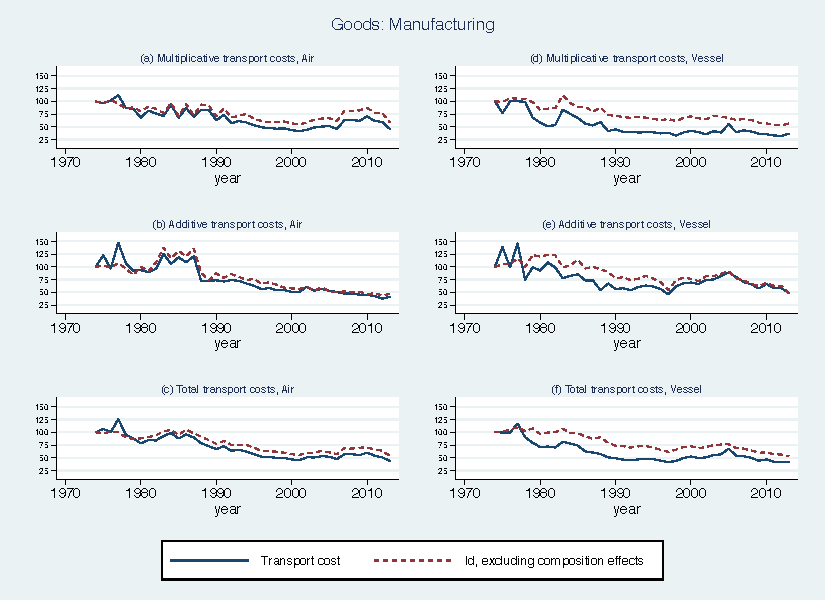
\includegraphics[height=8cm]
{graph_composition_manuf.pdf}
\end{center}
\end{figure}

\begin{figure}[htbp]
\caption{Transport costs (with and without composition effects), Primary goods}
\label{fig:totalTC_compeffects_excl_primary}
\begin{center}
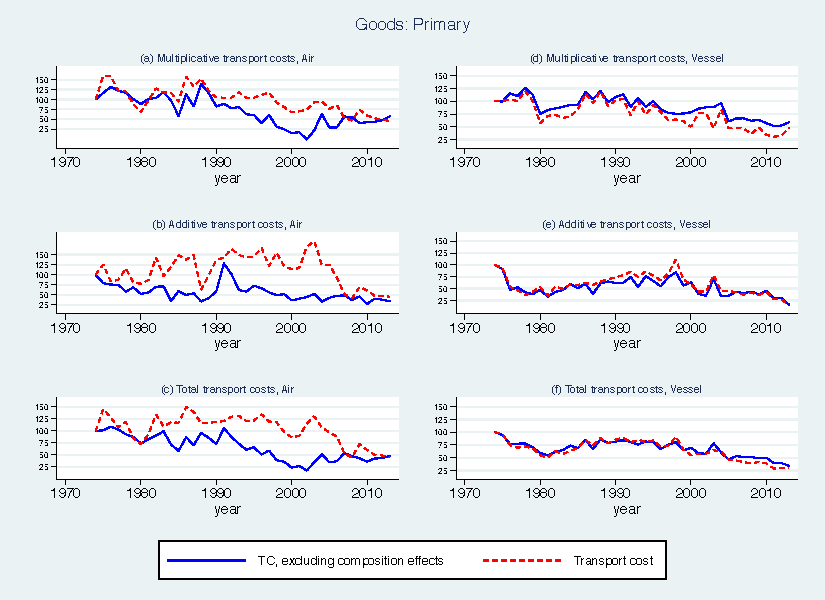
\includegraphics[height=8cm]
{graph_composition_primary.pdf}
\end{center}
\end{figure}

\begin{figure}[htbp]
\caption{Transport costs (with and without composition effects)}
\label{fig:totalTC_compeffects_excl}
\begin{center}
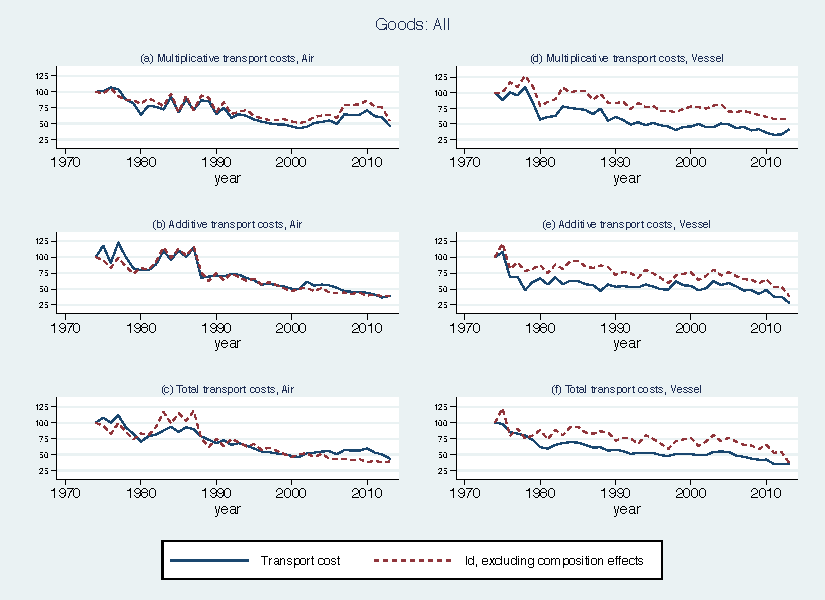
\includegraphics[height=8cm]
{graph_composition_all.pdf}
\end{center}
\end{figure}

As reported in Figures \ref{fig:totalTC_compeffects_excl_manuf} and \ref{fig:totalTC_compeffects_excl_primary}, the ``raw'' transport costs are (or the unfitted transport costs, in plain blue line) have regularly declined over the period in both sectors, by roughly the same order of magnitude (50\% in Air, 60\% in Vessel). However, contrasting these two broad sectors conveys a contrasted message about the role of trade composition effects in accounting for this trend pattern. Comparing Figure \ref{fig:totalTC_compeffects_excl_manuf} reports a very similar time trend decomposition than what is obtained on the whole range of goods (Figure \ref{fig:totalTC_compeffects_excl}). In Air transport, most of the decrease can be imputed to the reduction of``ceteris paribus'' transport costs (the dotted red line), trade composition effects playing virtually no role (Figure \ref{fig:totalTC_compeffects_excl_manuf}, left-hand panels (a), (b) and (c)). Trade composition effects matter more in maritime transport (Figure \ref{fig:totalTC_compeffects_excl_manuf}, right-hand panels (d), (e) and (f)), primarily in the ad-valorem component. Similarly as the conclusion drawn on the whole range of flows, the 60\% decrease in the unfitted transport costs in Vessel can de decomposed in a 50\% decrease in the ``ceteris paribus'' transport costs (fitted), the 10\% remaining to trade composition effects.

The message is strikingly different when the same decomposition is driven for primary goods only. In this case, it is in air transport that composition effects do matter (Figure \ref{fig:totalTC_compeffects_excl_primary}, left-hand panels (a), (b) and (c)), while we observe not much role for them in maritime transport (Figure \ref{fig:totalTC_compeffects_excl_primary}, left-hand panels (d), (e) and (f)). In air transport further, composition effects matter by partially offsetting the decrease in the ``ceteris paribus'' transport costs (ie, implying a reduction in the ``raw'' transport costs over time much less pronounced than the fitted transport cost measures).

One way to reconcile the contrasted results displayed in Figure \ref{fig:totalTC_compeffects_excl_primary} (primary goods), with respect to Figure \ref{fig:totalTC_compeffects_excl_manuf} (manufacturing) and Figure \ref{fig:totalTC_compeffects_excl} (all flows) is to investigate the share of primary goods in total flows. The results are reported in Figure \ref{fig:Share_prim_goods}. In Air transport, the share of primary goods in the total value of US imports is negligible, by around 10\% all over the period from 1974 to 2004. Primary goods make a higher proportion of trade flows in maritime transport, especially over 1974-1982 (between 40\% and 60\%). On the following sub-period though, their share has fallen to 20-30\%. Given the modest proportion of primary goods in total imports flows of the US economy, in favor of the manufactured sector, it is hence not surprising that the diagnosis made about the time trend of transport costs when all types of flows are considered, is driven by the trend patterns that occur within the manufacturing sector.


\begin{figure}[htbp]
\caption{Share of primary goods in the value of total US imports}
\label{fig:Share_prim_goods}
\begin{center}
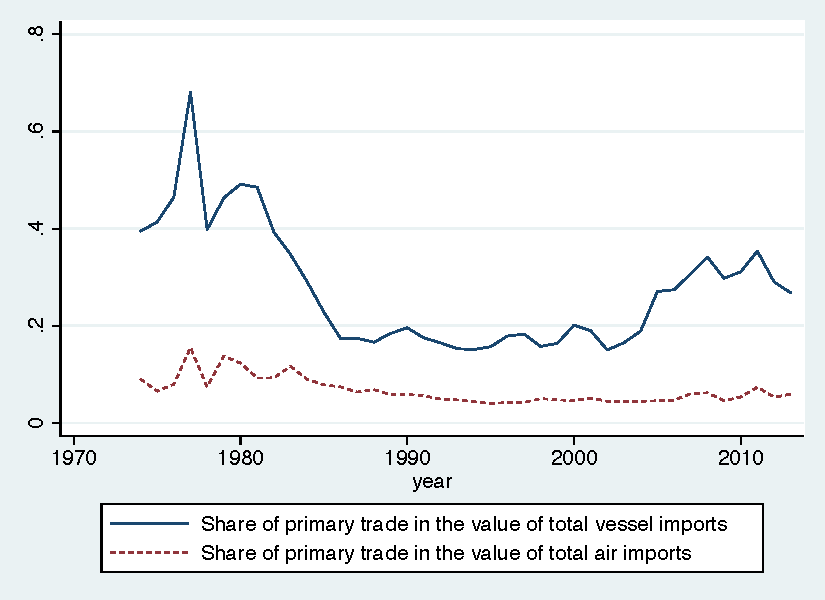
\includegraphics[height=6cm]
{Share_of_primary.pdf}
\end{center}
\end{figure}



\end{document}
